\section {Design and Implementation\\}

\subsection{Reactor Model\\}
The PushUp Server runs atop of the Twisted framework\cite{Twisted}, which 
adopts the reactor model\cite{Reactor} to enable event-driven mechanism. 

The Reactor patterns involve synchronous I/O. In this pattern the event 
demultiplexor waits for events (for example, file descriptor is 
ready for a write operation), The demultiplexor passes this event to the
appropriate event handler(implemented as the callback), which is 
responsible for performing the actual read or write.

In our case the Reactor is implemented as event loops(one Reactor 
can start several event loops) that runs in a single thread. The
event loop in twisted has well encapsulated the OS's underlying 
event notification mechanism (kqueue() in Unix and epoll() in Linux).
During execution, the event loop manages the details event handler 
registrations for particular event types, the activations of event 
handlers as events occur, etc.

Figure \ref{fig:eventloop} demonstrates the how the execution switches
between the event loops and user code. Figure \ref{fig:eventloop_flow} 
further illustrates the detailed work flow with sequence diagram.

As we can see from these figures, one of the caveat of in 
event-driven programming is that each event handler should 
be carefully design in order to make sure its execution 
will not take a long time; otherwise the whole system will 
be blocked.

\begin{figure}[htb!]
    \centering%
    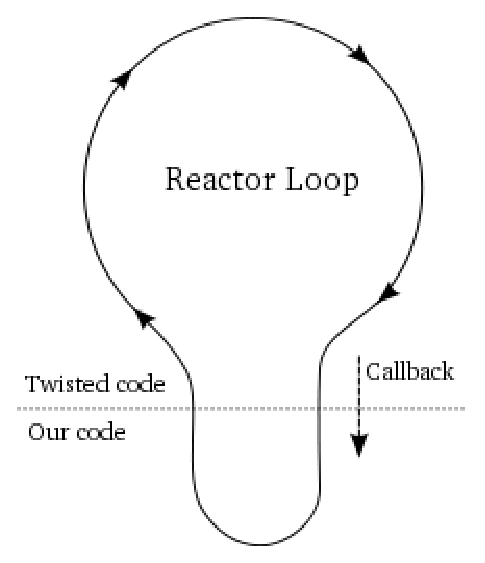
\includegraphics[scale=0.75]{figures/mainloop.eps}
    \caption{Work flow of Twisted Reactor Model}
    \label{fig:mainloop}
\end{figure}
\begin{figure}[htb!]
    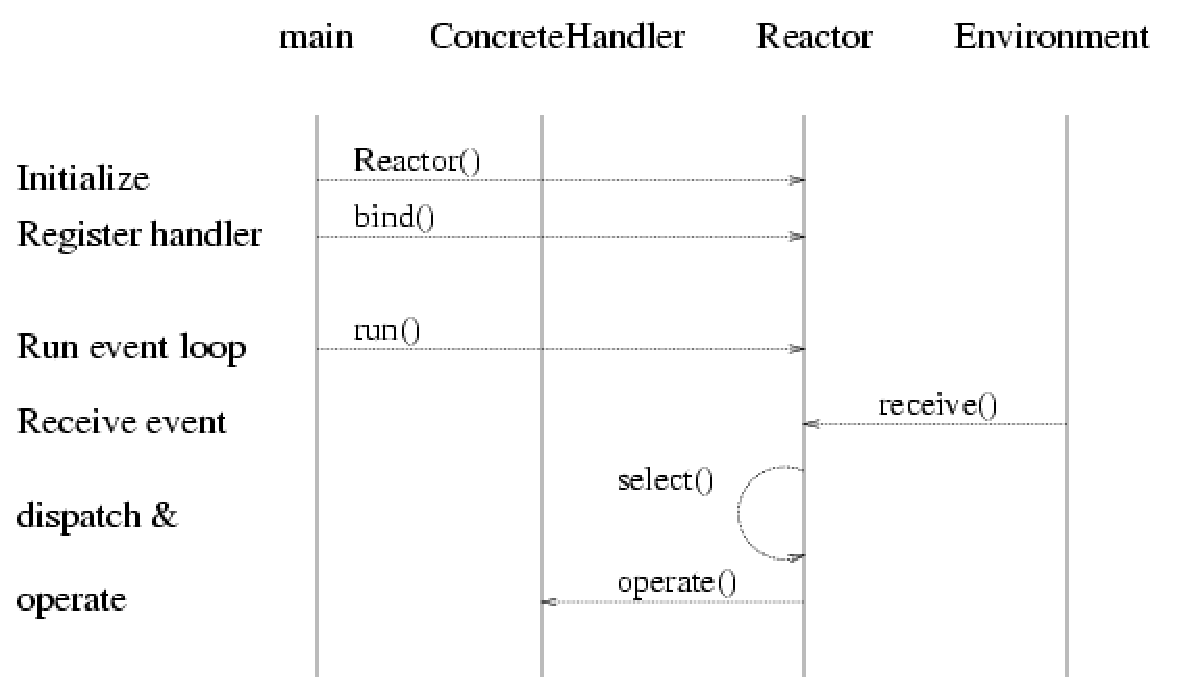
\includegraphics[scale=0.50]{figures/eventloop_flow.eps}
    \caption{The Sequence Diagram of the Event Loop}
    \label{fig:eventloop_flow}
\end{figure}


\subsection{Reverse Proxy\\}

How it works, with more details.

\subsection{Message Queue\\}

Pub/Sub: with more details

Publisher: 

    * General design

    * Backend sever connect to the 

Subscriber: 

    * General Design

    * Client Design

    * Just 50 seconds

Message Management

Subscriber

Internal Data structure: what are the highlight of such design.

\subsection{Load Balancer\\}

HAProxy -- driven on xxxx.

